\section{Fluxional execution model} \label{section:model}

The tool we present in this paper transforms a monolithic application into a network of autonomous parts communicating with message streams.
There exist many execution models designed for such distributed system renowned precisely for their performances\cite{Welsh2000, Jain2006, Wu2007, Zaharia2010, Akidau2013, Marz2011}.
However, we focus on the shift in programming model rather than the performance of the runtime.
Therefore, we present in this section an extremely simplified execution model inspired by the literature, only to support the confirmation of feasibility for the compilation process detailed in section \ref{section:compiler}.

\subsection{Fluxions}

The fluxional execution model role is to manage and invoke autonomous execution units.
An execution unit listens for, and sends back streams.
A stream is a continuous and infinite sequence of data encapsulated in messages.
We named this execution unit a fluxion, by contraction between a flux and a function.
A fluxion is a function, as in functional programming, only dependent on input and output streams.
It is composed of a unique name, a processing function, and a persisted memory \textit{context}.

Messages are carried between fluxions by a messaging system.
They are composed of the name of the recipient fluxion and a body.
At a message reception, the fluxion modifies its memory \textit{context}, and sends back messages to downstream fluxions.
The fluxion's memory \textit{context} contains all of the state variables on which the fluxion depends between two executions - that is two messages receptions.

The fluxions form a chain of processing binded by data streams.
All these chains constitute a directed graph, operated by the messaging system.

\subsection{Messaging system}

The messaging system is the core of our fluxional execution model.
It carries messages along streams, and invokes fluxions at a message reception.

The messaging system is built around a message queue.
Each message is processed one after the other by invocation of the destination fluxion.
% Using a message queue allows to execute multiple processing chains fairly and concurrently, without difference in scheduling local messages, or network messages.
The life cycle of a fluxional application is pictured on figure \ref{fig:MesSys}.

\begin{figure}[h!]
  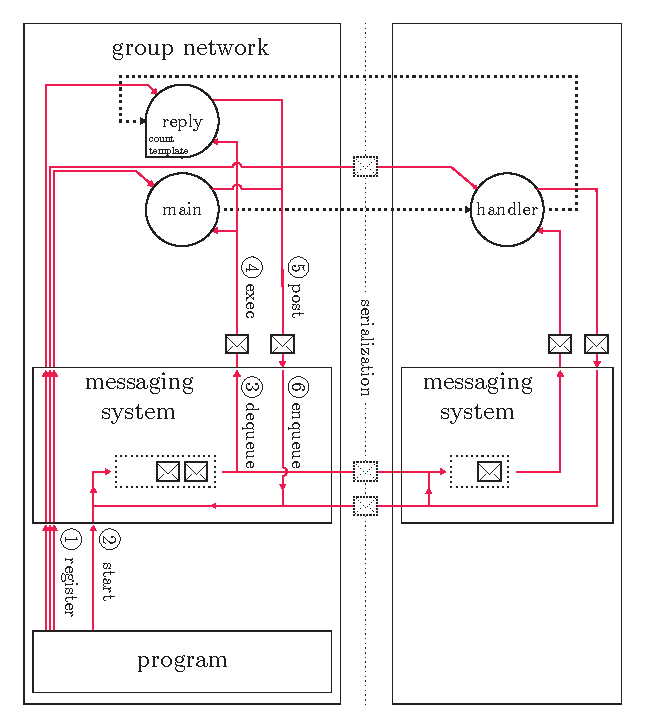
\includegraphics[width=\linewidth]{ressources/schema-message.pdf}
  \caption{Messaging system details}
  \label{fig:MesSys}
\end{figure}

The messaging system carries message streams based on the names of the recipient fluxions.
So it needs every fluxion to be registered.
If two fluxions share a name, the messaging system would be in a conflicting situation.
This registration associates a processing function with a unique name and an initial memory \textit{context}.
The registration is done using the function \texttt{register(<nom>, <fn>, <context>)}, step \circled{1} on figure \ref{fig:MesSys}.
% A fluxion can dynamically register other fluxions

To trigger a chain of fluxions, a message is sent using the function \texttt{start(<msg>)}, step \circled{2}.
This function pushes a first message in the queue.
Immediately, the system dequeues this message to invoke the recipient processing function, step \circled{3} and \circled{4}.
The recipient function sends back messages using the function \texttt{post(<msg>)}, step \circled{5}, to be enqueued in the system, step \circled{6}.
The system loops through steps \circled{3} and \circled{4} until the queue is empty.
This cycle start again for each new start.

The algorithms \ref{alg:parcours} and \ref{alg:traitement} precisely describe the behavior of the messaging system after the function \texttt{start} invocation.

\begin{algorithm}
\caption{Message queue walking algorithm}
\label{alg:parcours}
\begin{algorithmic}
\Function{loopMessage}{\null}
\While{$msg$ \textbf{presents in} $msgQueue$}
\State $msg \gets$ \Call{dequeue}{\null} \Comment{\circled{3}}
\State \Call{ProcessMsg}{$msg$}
\EndWhile
\EndFunction
\end{algorithmic}
\end{algorithm}

\begin{algorithm}
\caption{Message processing algorithm}
\label{alg:traitement}
\begin{algorithmic}
\Function{processMsg}{$msg$}
\For{$dest$ \textbf{in} $msg.dest$}
\State $fluxion \gets lookup(dest)$
\State $message \gets$ \Call{exec}{$fluxion, msg.body$} \Comment{\circled{4} \& \circled{5}}
\State \Call{enqueue}{$message$} \Comment{\circled{6}}
\EndFor
\EndFunction
\end{algorithmic}
\end{algorithm}

% \subsection{External interfaces}

% In order to interact with other systems, we define external border interfaces.
% As a first approach, our goal is to interface Web architectures, so we need to communicate with a REST\cite{Fielding2002} client.
% We define two components in this interface :

% \begin{itemize}
% 	\item[\textbf{In}]
%     receives client connections.
%     % This is so the first link in the chain.
%     For every incoming connection, it relays a connection identifier to the \textbf{Out} component for the reply.
%     It then relays the connection identifier and the request to the first fluxion by calling the \texttt{start} function.
% 	\item[\textbf{Out}]
%     sends the result of the processing chain back to the client.
%     To receive messages from the processing chain, the component \textbf{Out} is registered in the messaging system under the name \texttt{out}.
%     % This is so the last link in the chain.
% \end{itemize}

% Figure \ref{fig:schemaweb} pictures the specific elements of the web interface inside the fluxional system.
% % La figure \ref{fig:schemaweb} illustre les éléments spécifiques de cette interface Web au sein du système fluxional illustré par la figure \ref{fig:MesSys}.

% \begin{figure}[h!]
% 	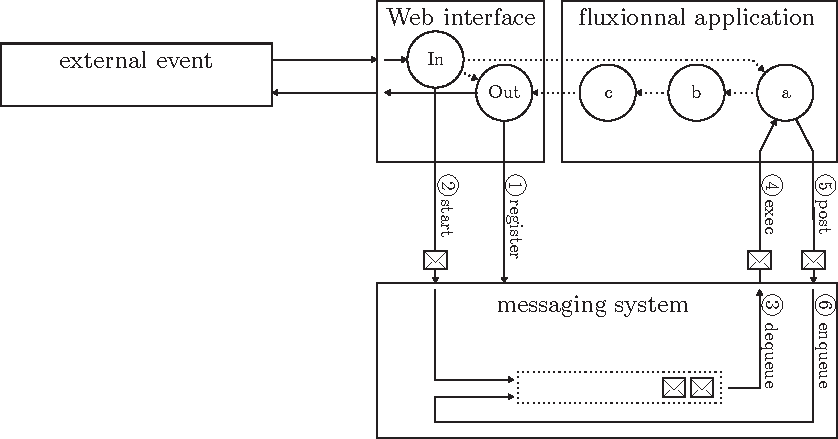
\includegraphics[width=\linewidth]{ressources/schema-web.pdf}
% 	\caption{Fluxional application with web interface}
% 	\label{fig:schemaweb}
% \end{figure}

% TODO paragraphe de transition

\subsection{Service example}

In order to picture the fluxional execution model, we present an example of a simple web application.
This application sends back its own source along with a download counter.

\includecode{js,
  caption={Source of the compilation example},
  label={lst:ex-source}
}
{../../example/source.js}

% \begin{code}[js, caption={Original code of a simple service example},label={lst:classique}]
% var app = require('express')();

% @\label{lst:classique_count}@var count = {};

% @\label{lst:classique_get}\label{lst:classique_replyb}@app.get('/:id', function reply(req, res){
%   count[req.params.id] = count[req.params.id]  || 1; @\label{lst:classique_dynres}@
%   ++count[req.params.id] 
%   var visits = count[req.params.id];
%   var reply = req.params.id + ' connected ' + visits + ' times.';
% @\label{lst:classique_send}@  res.send(reply);
% @\label{lst:classique_replye}@});

% port = 8080;
% app.listen(port);
% console.log("Listening port: "+port);
% \end{code}

% The initial version of this service could look like code listing \ref{lst:classique}.
The original source code of this application is available on github\cite{flx-example}\footnote{\raggedright https://github.com/etnbrd/flx-example/releases}, and in listing \ref{lst:ex-source}.
In this source code, some points are worth noticing.

\begin{itemize}
  \item The \texttt{reply} function, line 5 to 11, contains the logic we want to split into the fluxional processing chain.
  It receives the user request in the variable \texttt{res} which is used in the whole chain.
  \item The \texttt{count} object at line 3 is a persistent memory that increment the download counter.
  This object needs to be mapped to a fluxion \textit{execution context} in the fluxional system.
  \item The two functions \texttt{get} and \texttt{send}, respectively line 5 and 9, interface the application with the clients.
  The processing chain of functions is in between these two functions : $\texttt{get} \to \texttt{handler} \to \texttt{readFile} \to \texttt{reply} \to \texttt{send}$.
\end{itemize}

This minimal application is transformed manually into the fluxions chain depicted in Figure \ref{fig:fluxions}.
We expect a similar result with the compiler described in next section.
The circles represent registered fluxions.
Envelope symbols represent messages streams between fluxions with the data transmitted from one fluxion to the other.
The square in the messaging system hold the memory \textit{context} of the \texttt{reply} fluxion.
When a new \texttt{GET} REST request is received by the starting fluxion named \texttt{get}, a \texttt{start} message triggers the flow.
The \texttt{handler} fluxion receives this \texttt{start} message, read the source file and forward it to the \texttt{reply} fluxion which increments the counter, and sends the result back.
Each fluxion propagates the necessary values from one fluxion to the other exclusively by messages.
Horizontal dashed lines show message virtual transmission between fluxions although they all go through the messaging system.

\begin{figure}[h!]
  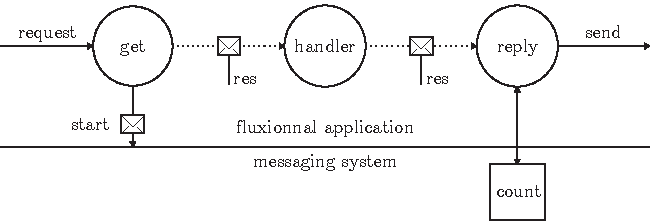
\includegraphics[width=\linewidth]{ressources/flux.pdf}
  \caption{Count service fluxions chain}
  \label{fig:fluxions}
\end{figure}

Listing \ref{lst:fluxional} describes this counting application in our high-level fluxional language.
This language brings a stricter segmentation than the initial code by allowing to only define and register fluxions.
% And so, it allows an additional system to optimize the organization of the system on different physical machines according to the cost of fluxions' streams and processing.
In this language, a fluxion is defined by a name, a description of the memory \textit{context}, the operator \texttt{>}\texttt{>} for starting fluxions or \texttt{-}\texttt{>} for following fluxions and finally a list of downstream fluxions with the content of the message for each stream.
Following the fluxion definition is the body containing the processing function, using the Javascript language syntax.
The processing function can access and manipulate only two objects : \texttt{msg} and \texttt{this}.
The first is the received message, the second is the persisted context of the fluxion.
There is an exception for the starting fluxion whose body doesn't contains a function, because it never receives any stream, but only initializes the application.

% This high level language is not dynamic, and not typed.
% You can register fluxion at any time, and the messages can contain any type or composition of types.
% \TODO{write a paragraph about the languages characteristics, a reserved subsection might be necessary, but maybe better placed in the next section, about transformation}

% \begin{code}[js, caption={Fluxional sample},label={lst:fluxional}]
% use web

% fluxion logic -> view
%   this.uid[msg.uid] = this.uid[msg.uid] + 1 || 1
%   msg.count = this.uid[msg.uid]
%   post msg

% fluxion view -> output
%   msg.view = msg.uid + " connected " + msg.count + " times."
%   msg.uid = undefined
%   msg.count = undefined
%   post msg

% register logic, {uid: {}}
% register view

% web.listen
% \end{code}

\begin{code}[flx, caption={Fluxional sample},label={lst:fluxional}]
flx get
>> handler [res]
  var app = require('express')(),
      fs = require('fs'),
      count = 0;

  app.get('/', >> handler);
  app.listen(8080);
  console.log('>> listening 8080');

flx handler
-> reply [res]
  function handler(req, res) {
    fs.readFile(__filename, -> reply);
  }

flx reply {count}
-> null
  function reply(error, data) {
    count += 1;
    var code = ('' + data).replace(/\n/g, '<br>').replace(/ /g, '&nbsp');
    res.send('downloaded ' + count + ' times<br><br><code>' + code + '</code>');
  }
\end{code}

The application is organized as follow :
\begin{itemize}
  \item The \texttt{get} fluxion is the starting fluxion.
  It initialize the application to listen for user request calling \texttt{app.get}.
  Every request is sent to the \texttt{handler} request.
  \item The \texttt{handler} fluxion read the source file to send it to the user, and forward the result to the \texttt{reply} fluxion.
  \item The \testtt{reply} fluxion increments the counter, formats the reply, and sends it back to the user using the function \texttt{res.send}.
\end{itemize}

We use this interface to develop web services using the fluxional execution model.
But our goal, as described in the introduction, is to automate this architecture shift, not to impose a new programming paradigm onto the developer.
% We now evaluate this model against the basic one.


